\documentclass[proseminar,german,utf8]{zihpub}
\usepackage{setspace}
\usepackage{hyperref}
\usepackage{graphicx}

\author{Paul Gottschaldt}
\title{Julia - High-Performance Programmiersprache für High-Performance Computing?}
\matno{4609055}
\betreuer{Martin Schroschk}
\bibfiles{}
\copyrighterklaerung{Hier soll jeder Autor die von ihm eingeholten
Zustimmungen der Copyright-Besitzer angeben bzw. die in Web Press
Rooms angegebenen generellen Konditionen seiner Text- und
Bild\"ubernahmen zitieren.}
\acknowledgments{Die Danksagung...}

\begin{document}
\section {Einleitung}
1998 startete das Apache-Point-Observatorium in New Mexico ihr Projekt Sloan Digital Sky Survey (SDSS), welches Fotos von über 35\% aller sichtbaren Objekte unseres Himmels anfertigte und in einer Datenbank zunächst sicherte. Seit diesem Jahr wurden bereits über 500 Millionen Sterne und Galaxien fotografiert und Licht eingefangen, welches bereits Milliarden von Jahren unterwegs war und uns bis weit in die Vergangenheit unseres Universums zurückblicken lässt. Die SDSS Kamera galt als produktivste Weltraumkamera der Welt bis zu ihrer Abschaltung im November 2009. Mit etwa 200 GB reine Bilddaten pro Nacht entstand so eine Datenbank mit über 5 Millionen Bildern von jeweils 12 Megabyte - zusammengerechnet also rund 55 Terabyte\footnote{\url{https://juliacomputing.com/press/2016/11/28/celeste.html}}. 2014 startete ein Team von Astronomen, Physikern, Informatikern und Statistikern das Projekt Celeste um eben jenen Datensatz zu katalogisieren und für jeden Himmelskörper einen Eintrag anzulegen\footnote{\url{https://juliacomputing.com/case-studies/celeste.html}}. In der ersten veröffentlichten Version von 2015 noch auf Berechnungen auf einzelne Knoten beschränkt, schaffte es das Forschungsteam um die involvierten Parteien Julia Computing, UC Berkeley, Intel, National Energy Research Scientific Computing Center (NERSC) und Lawrence Berkeley National Laboratory in der 2. Version von 2016 bereits einen 225-fachen Geschwindigkeitsgewinn zu erzielen. Die größten Verbesserungen waren dabei der mit 8192 Intel® Xeon® Prozessoren ausgestattete HPC des Berkeley Lab's und Julia, eine High-Performance Open-Source Programmiersprache, die bis dato noch relativ unbekannt war und seit 2009 am MIT entwickelt wird. Besonders ist an Julia vorallem ihr Anspruch, eine sehr produktive (high-programming language) wie Python zu sein, dabei aber Geschwindigkeiten wie C zu erreichen. Im November 2017 veröffentlichte dieses Team dann die aktuelle 3. Version, mit der sie nochmals einen deutlichen Geschwindigkeitsgewinn erreichen konnten. Sie schafften es 188 Millionen Sterne und Galaxien in nur 14.6 Minuten zu katalogisieren und nutzten dafür bis zu 1.3 Millionen Threads auf den 9300 Knights Landing(KNL) Knoten des Cori Supercomputers des NERSC. Dabei erzielten sie mit Julia eine Peak-Performance von 1.54 PetaFlop/s für Gleitkommaberechnungen mit doppelter Genauigkeit. Damit erzielt das Celeste Projekt einen 100-fachen Gewinn zu allen vorherigen Forschungsprojekten. Derzeit gibt es rund 200 Supercomputer in der Welt, welche in der Lage sind eine Peak-Performance von mehr als einem Petaflop pro Sekunde zu erreichen. Trotzdem sind so gut wie alle Anwendungen, welche eben jene Peak-Performance erreichen von einer Gruppe von Ninjas geschrieben, welche ein sehr tiefes Verständnis für alle erforderlichen Details besitzen, die man benötigt um solch eine Performance zu erreichen\footnote{\url{https://www.nextplatform.com/2017/11/28/julia-language-delivers-petascale-hpc-performance/}}. Umso erstaunlicher ist an diesem Ergebnis also die Tatsache, dass das Team hinter Celeste ihre Geschwindigkeit ausschließlich unter Nutzung ihrer Kenntnisse, dem Juliacode und dessen Threading Model erzielen konnten.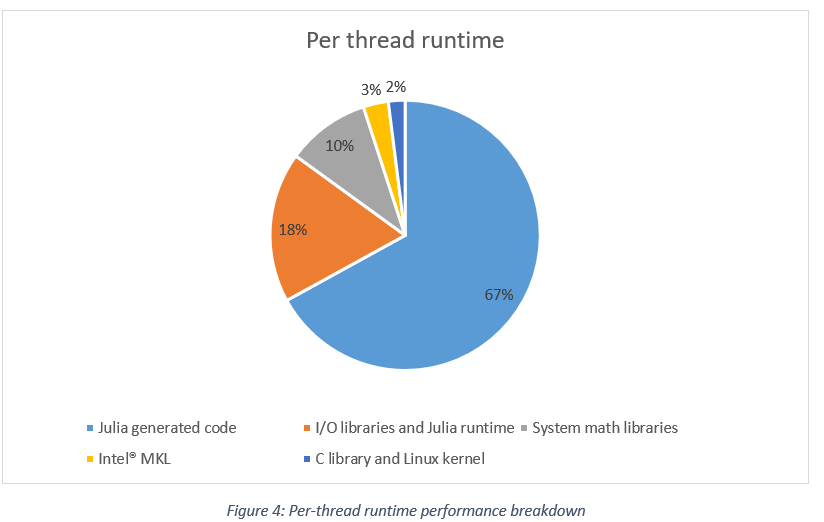
\includegraphics[scale=0.5]{celestejulia.png}  Wie in der Übersicht zur pro Thread Auslastung zu sehen, lieferte Julia 82.3\% der Performance. Damit stellt Julia unter Beweis das es sowohl für ThetaByte-große Datensätze, wie auch für PetaByte-schnelle Berechnungen geeignet ist. Keno Fischer, CTO von Julia Computing, sagte 2017, das Projekte wie Celeste unter Beweis stellen, das der Traum, der hinter Julia steht, wahr wird. Wissenschaftler können nun auf ihrem Rechner entwickelte Prototypen einfach von ihrem Laptop auf die größten Supercomputer verschieben ohne zwischen Sprachen wechseln zu müssen oder ihren Code gar komplett neu zu schreiben. Sie (Anmerkung: Entwickler von Julia Computing) sind sehr stolz darauf, dies alles geschafft zu haben und glauben sehr daran, das Julia die Entwcklung in der Forschung für viele Jahre sehr voranbringen wird. Viral Shah, CEO von Julia Computing, sagte das Forscher sich nun auf die Lösung ihrer Probleme fokussieren können und sich nicht mehr mit dem Programmieren beschäftigen müssen\footnote{\url{https://juliacomputing.com/press/2016/11/28/celeste.html}}.
%%%%%%%%%%%%%%%%%%%%%%%%%%%%%%%%%%%%%%%%%%%%%%%%%%%%%%%%%%%%%%%%%%%%%%%

\section{Einführung in die Programmiersprache Julia}
\subsection{Julia, die dynamische, stark typisierte funktionale Programmiersprache}
Julia ist eine junge, flexible, höhere Programmiersprache die es sich selbst als Ziel gesetzt hat, die hohe Produktivität und einfache Handhabbarkeit aus Sprachen wie Python mit der Geschwindigkeit von C zu kombinieren. Auch wenn sie vorallem für wisssentschaftliches und numerisches Programmieren gestaltet worden ist, bietet sie eine sogleich performante wie auch einfach zu lernende Umgebung und versucht damit den derzeitigen Trend von mehrsprachigen Softwarelösungen in der Wissenschaft entgegen zu wirken. Mit einem Syntax der an eine Kombination aus MATLAB und Python erinnert, Lisp ähnlichen Macros und Metaprogrammierung, einem Compiler der LLVM nutzt und einem eigenem Paketmanager der an Git erinnert, hat sich Julia viele bereits etablierte Funktionen zunutze gemacht. Zusätzlich besitzt sie die Möglichkeit C und Python Funktionen einfach direkt aufzurufen was die Nutzung der Bibliotheken der beiden Sprachen direkt im Julia Code ermöglicht. Julias gute Performance wird vorallem durch Multimethoden für einzelne Funktionen und die automatische Generierung von effizientem typspezialisierten Code gewonnen. Dabei ist Julia sowohl dynamisch wie auch statisch typisiert. Zudem ist Julia funktional, objektorientiert und imperativ und wurde fast komplett in Julia selbst geschrieben.
\subsection{Julias Typensystem und Multimethoden}

\section{Parallele Programmierung mit Julia}
\section{Bewertung der HPC-Eignung von Julia}
\section{Quellen}
\subsection{Links}
Links für die Einleitung:
\begin{itemize}
\item https://juliacomputing.com/case-studies/celeste.html am 14.05.18 um 14:52 Uhr
\item https://www.heise.de/developer/meldung/Programmiersprache-Julia-profiliert-sich-beim-High-Performance-Computing-3518621.html am 14.05.18 um 14:52 Uhr
\item https://github.com/jeff-regier/Celeste.jl am 14.05.18 um 14:52 Uhr
\item https://www.youtube.com/watch?v=uecdcADM3hY am 14.05.18 um 14:52 Uhr
\item https://juliacomputing.com/press/2016/11/28/celeste.html am 14.05.18 um 14:52 Uhr
\item https://de.wikipedia.org/wiki/Sloan\_Digital\_Sky\_Survey am 14.05.18 um 14:53 Uhr
\item https://de.wikipedia.org/wiki/Apache\-Point\-Observatorium am 14.05.18 um 14:53 Uhr
\item http://www.astronews.com/news/artikel/2014/01/1401-013.shtml am 14.05.18 um 14:54 Uhr
\item http://www.sdss.org/dr14/imaging/ am 14.05.18 um 14:54 Uhr
\item https://www.nextplatform.com/2017/11/28/julia-language-delivers-petascale-hpc-performance/ am 14.05.18 um 14:54 Uhr
\end{itemize}

Links für die Definition:
\begin{itemize}
\item https://julialang.org/ am 14.05.18 um 14:57 Uhr
\item https://www.heise.de/developer/artikel/Funktionsorientiert\-und\-schnell\-Die\-Programmiersprache\-Julia\-3793160.html?seite=all am 14.05.18 um 14:58 Uhr
\item https://de.wikipedia.org/wiki/Julia\_\(Programmiersprache\) am 14.05.18 um 14:58 Uhr
\item https://docs.julialang.org/en/stable/manual/introduction/\#man-introduction\-1 am 14.05.18 um 14:59 Uhr
\end{itemize}


\end{document}
